\section{Classification} \label{sec:chp2-sec6}
The classification problem was discussed previously in Sect.~\ref{sec:chp2-sec1}.
%We discussed and introduced the classification problem previously in Sect.~\ref{sec:chp2-sec1}. 
Numerous approaches have been introduced by the research community to solve the classification problem. 
%Here we will discuss some of these approaches under two categories of single learner and ensemble. 
Here we discuss some of these approaches divided into two categories: ``single learner'' and ``ensemble''.  

\subsection{Single Learner}
This group contains a large number of classifiers, or base learners, that have a unique approach to learn from the training set. 
In the following, we discuss some of these classifiers: \ac{svm}, K-\ac{nn}, \ac{lda} and \ac{nb}. 

\begin{description}

\item[\acf{nb}] is one of the simplest probabilistic classifiers, based on Bayes' theorem. 
This classifier has a ``naive'' or independence assumption that states that features are conditionally independent given the class variable~\cite{murphy2012machine}. 
Given a sample to be classified represented by $n$ features, $\mathbf{x} = (x_{1}, ..., x_{n})$, the conditional probability of this sample belonging to class $C_{k}$ based on Bayes' theorem is given by: 
\begin{equation}
p(C_{k}|\mathbf{x}) = \frac{p(C_{k})p(\mathbf{x}|C_{k})}{p(\mathbf{x})}.
\label{eq:BT}
\end{equation}
This equation simply states that the posterior is equal to the prior times the likelihood while normalized.
Considering that the numerator of Eq.~\ref{eq:BT} can be written as a joint probability $p(C_{k}, x_{1}, ..., x_{n})$ and taking into account the conditional independence assumption, the \ac{nb} model is represented by: 
\begin{equation}
p(C_{k}|x_{1}, ..., x_{n}) = \frac{1}{Z}p(C_{k})\prod_{i =1}^{n} p(x_{i}|C_{k}),
\label{eq:nbM}
\end{equation} 
\noindent where $Z = p(x)$ is the normalization or scaling factor depending on $x_{1}, ...,x_{n}$.
For classification purposes, the \ac{nb} is combined with decision rules, such as \acf{map} or \acf{ml}: 
\begin{equation}
\hat{y} = \argmax_{k\in\{1,...,k\}} p(C_{k})\prod_{i=1}^{n} p(x_{i}|C_{k})~.
\end{equation}  

\item[K-Nearest Neighbor (k-\ac{nn})] is another simple and non-parametric classification method. 
This classifier assigns each sample's label based on the majority vote of its $K$ nearest neighbors. 
If $K$ is equal to 1, the output is assigned to the label of the nearest neighbor.
   
\item[\acf{lda}] or the Fisher linear discriminant analysis, was introduced in Sect.~\ref{sec:chp2-sec4} as a dimension reduction approach that takes the class label into account. 
Since this method contains the class information, it can be used for classification as well. 
However, it has a drawback, that regardless of the number of feature dimensions, it always maps the data to $L\leq C-1$. 
%Which indicates that for two class classification, it maps the data to one vector where the class margin is maximized~\cite{murphy2012machine}. 
This indicates that for a two class classification, in an attempt to maximize the margin between the two class, it maps the data to one vector~\cite{murphy2012machine}.

\item[\acf{svm}] is created based on the combination of the kernel trick and modified loss function~\cite{murphy2012machine}.
\ac{svm}~\cite{vapnik1963generalized} is a well known machine learning approach that aims to separate two classes by finding the best hyperplane maximizing the margin between the two classes: 
\begin{equation}
\min\limits_{\mathbf{w},\omega_{0}, \mathbf{\xi}} \frac{1}{2} \Vert \mathbf{w} \Vert^{2} + C \sum\limits_{i = 1}^{N} \xi_{i} \qquad \text{s.t. } \quad \xi_{i} \geq 0, \quad y_{i}(x_{i}^{T}\mathbf{w} + \omega_{0}) \geq 1 - \xi_{i}, i = 1:N .
\label{eq:svmop}
\end{equation}

Maximizing the margin is equivalent to minimizing the norm of the normal vector of the hyperplane: 
% Soft margine  no points should lie in the margin and can be solved as an optimization problem. 
\begin{equation}
\min\limits_{\mathbf{w}, \omega_{0}} \frac{1}{2} \Vert \mathbf{w}\Vert^{2} \qquad \text{s.t. } \quad  y_{i}(\mathbf{w}^{T}\mathbf{x_{i}} + \omega_{0}) \geq 1, i = 1: N.
\label{eq:svmsm}
\end{equation}
\noindent This constraint intends to force all the points to be on the correct side of the decision boundary (hyperplane) with a minimum distance of 1. 
This assumption is only valid if the data is linearly separable. 
Thus, for general cases, a slack variable $\xi_{i} \geq 0 $ is introduced. 
If the points are on/or inside the correct margin boundary, then $\xi_{i} = 0 $; if the points are inside the margin and still on the correct side of the decision boundary, then $0 < \xi_{i} \leq 1 $; otherwise, if the points lay on the wrong side of the decision boundary, $\xi_{i} > 1 $. 
This assumption introduces \textit{soft margin constraints}.
Considering the rule of $\xi_{i}$, the $\sum_{i} \xi_{i}$ term in Eq.~\ref{eq:svmop} describes the upper bound on the number of misclassified points and $C$ is the regularization parameter that controls the tolerance of the classifiers on the number of errors~\cite{murphy2012machine}. 
\end{description}  
   
\subsection{Ensemble}
Ensemble learners are defined by a combination of several base learners $f_{m}(.)$:
\begin{equation}
f(y|y, \pi) = \sum\limits_{m\in M} \omega_{m}f_{m}(y|x),
\label{eq:ensmeble}	
\end{equation} 
\noindent where $\omega_{m}$ is the tunable parameter~\cite{murphy2012machine}. 
Some ensembles are created based on the combination of base learners of the same type, such as \acf{rf} and \acf{adb}, whereas others combine different base learners in a specific way, e.g. stacking and \acf{ecoc}. 
Some well-known ensembles are described in the following. 

\begin{description}
\item[\acf{adb}] (short for Adaptive Boosting) is an ensemble learning algorithm that provides a high performance classifier via a linear combination of weak learners~\cite{freund1996experiments}.
Considering a training set $(x_{i}, y_{i})$, where $x$ is an $M$ dimensional feature vector and $y_{i}$ is its associated class label, \ac{adb} iteratively adds weighted weak learners ($\alpha_{t}h_{t}$) to assemble the final strong classifier.
Here, $\alpha_{t}$ is the weight and $h_{t}$ is the weak learner:
\begin{equation}
H(x) = sign (\sum\limits_{t =1}^{T} \alpha_{t}h_{t}(x))~.
\label{eq:adb}
\end{equation}
A weak learner is usually selected as a classifier that performs slightly better than randoms ($> 50\%$).
Weak learners are selected with their associated weight so that the sum of the training error $E_{t}$ of the resulting $t$ stage classifier is minimized. 
\begin{subequations}
\begin{align}
E_{t} &= \sum\limits_{i = 1}^{N} e^{-y_{i}H_{t}(x_{i})}~,\\
H_{t}(x) &= \alpha_{1}h_{1}(x) + ...+\alpha_{t}h_{t}(x)~.
\end{align}
\label{eq:adberror}
\end{subequations}
This ensemble is constructed with the aim of classifying harder patterns by re-weighting the distribution after each iteration~\cite{rokach2010ensemble}. 
Starting with equally distributed weights for our distribution $D_{1}(i) = 1/N, \quad i = 1: N$.
The distribution is updated after each iteration in a manner that the weights of correctly classified samples decrease and the weights of misclassified samples increase. 
\begin{equation}
D_{t+1}(i) = \frac{D_{t}(i).e^{-\alpha_{t}y_{t}h_{t}(x_{i})}}{Z_{t}}~.
\end{equation}
Re-weighting the distribution automatically forces the next weak learner to focus on the difficult samples.  
As mentioned previously, each weak learner is assigned a weight as well and the best weak learners have higher weights in comparison to the weakest learners.

A variety of learners can be adapted in the algorithm as weak learners such as neural networks or decision trees. 
One common weak learner is decision stump, which is a one-level decision tree, equivalent to the threshold that best splits the data.  
Each stump learner is characterized by three parameters: (i) the $m^{th}$ dimension of the features set where the classifier is applied, (ii) the decision level, i.e., the threshold splitting the data in the $m^{th}$ given dimension and (iii) the decision sign ($-$1 or +1) determining the inequality direction for the thresholding.
For a given batch of data with a set of features of size $M$, at each iteration of \ac{adb}, the decision stump that minimizes the error $t$ in an $m^{th}$ dimension of the training distribution is selected.
The information provided by the final set of decision stumps selected by \ac{adb} can also be used for determining the significant features of the data-stream and, more importantly the best split in the data.

\item[\acf{rf}] is an ensemble of decision trees~\cite{breiman2001random} that generalizes the classification process by applying two types of randomization: at the tree level, each tree is fed by a bootstrap made of $S'$ samples build from the original data of size $S$ so that  $S=S'$, and at the node level, a subset of feature dimensions $m$ is randomly selected from the original dimension $M$ so that $m=\sqrt{M}$. 
The trees in \ac{rf} are grown to their maximum length without any pruning.
Figure~\ref{fig:rftrain} shows the training stage of an \ac{rf} ensemble.
In this figure rows and columns represent the samples and the feature dimensions, respectively.
As it mentioned each tree is trained on the bootstrap of the original samples and in each node of a tree, subset of feature dimensions are used for prediction.  
In the testing stage, each tree in the ensemble casts a unit vote, and the final prediction is based on the combination of all the votes.
This process is shown in Fig~\ref{fig:rftest}.
\begin{figure}
\centering
\subfloat[]{
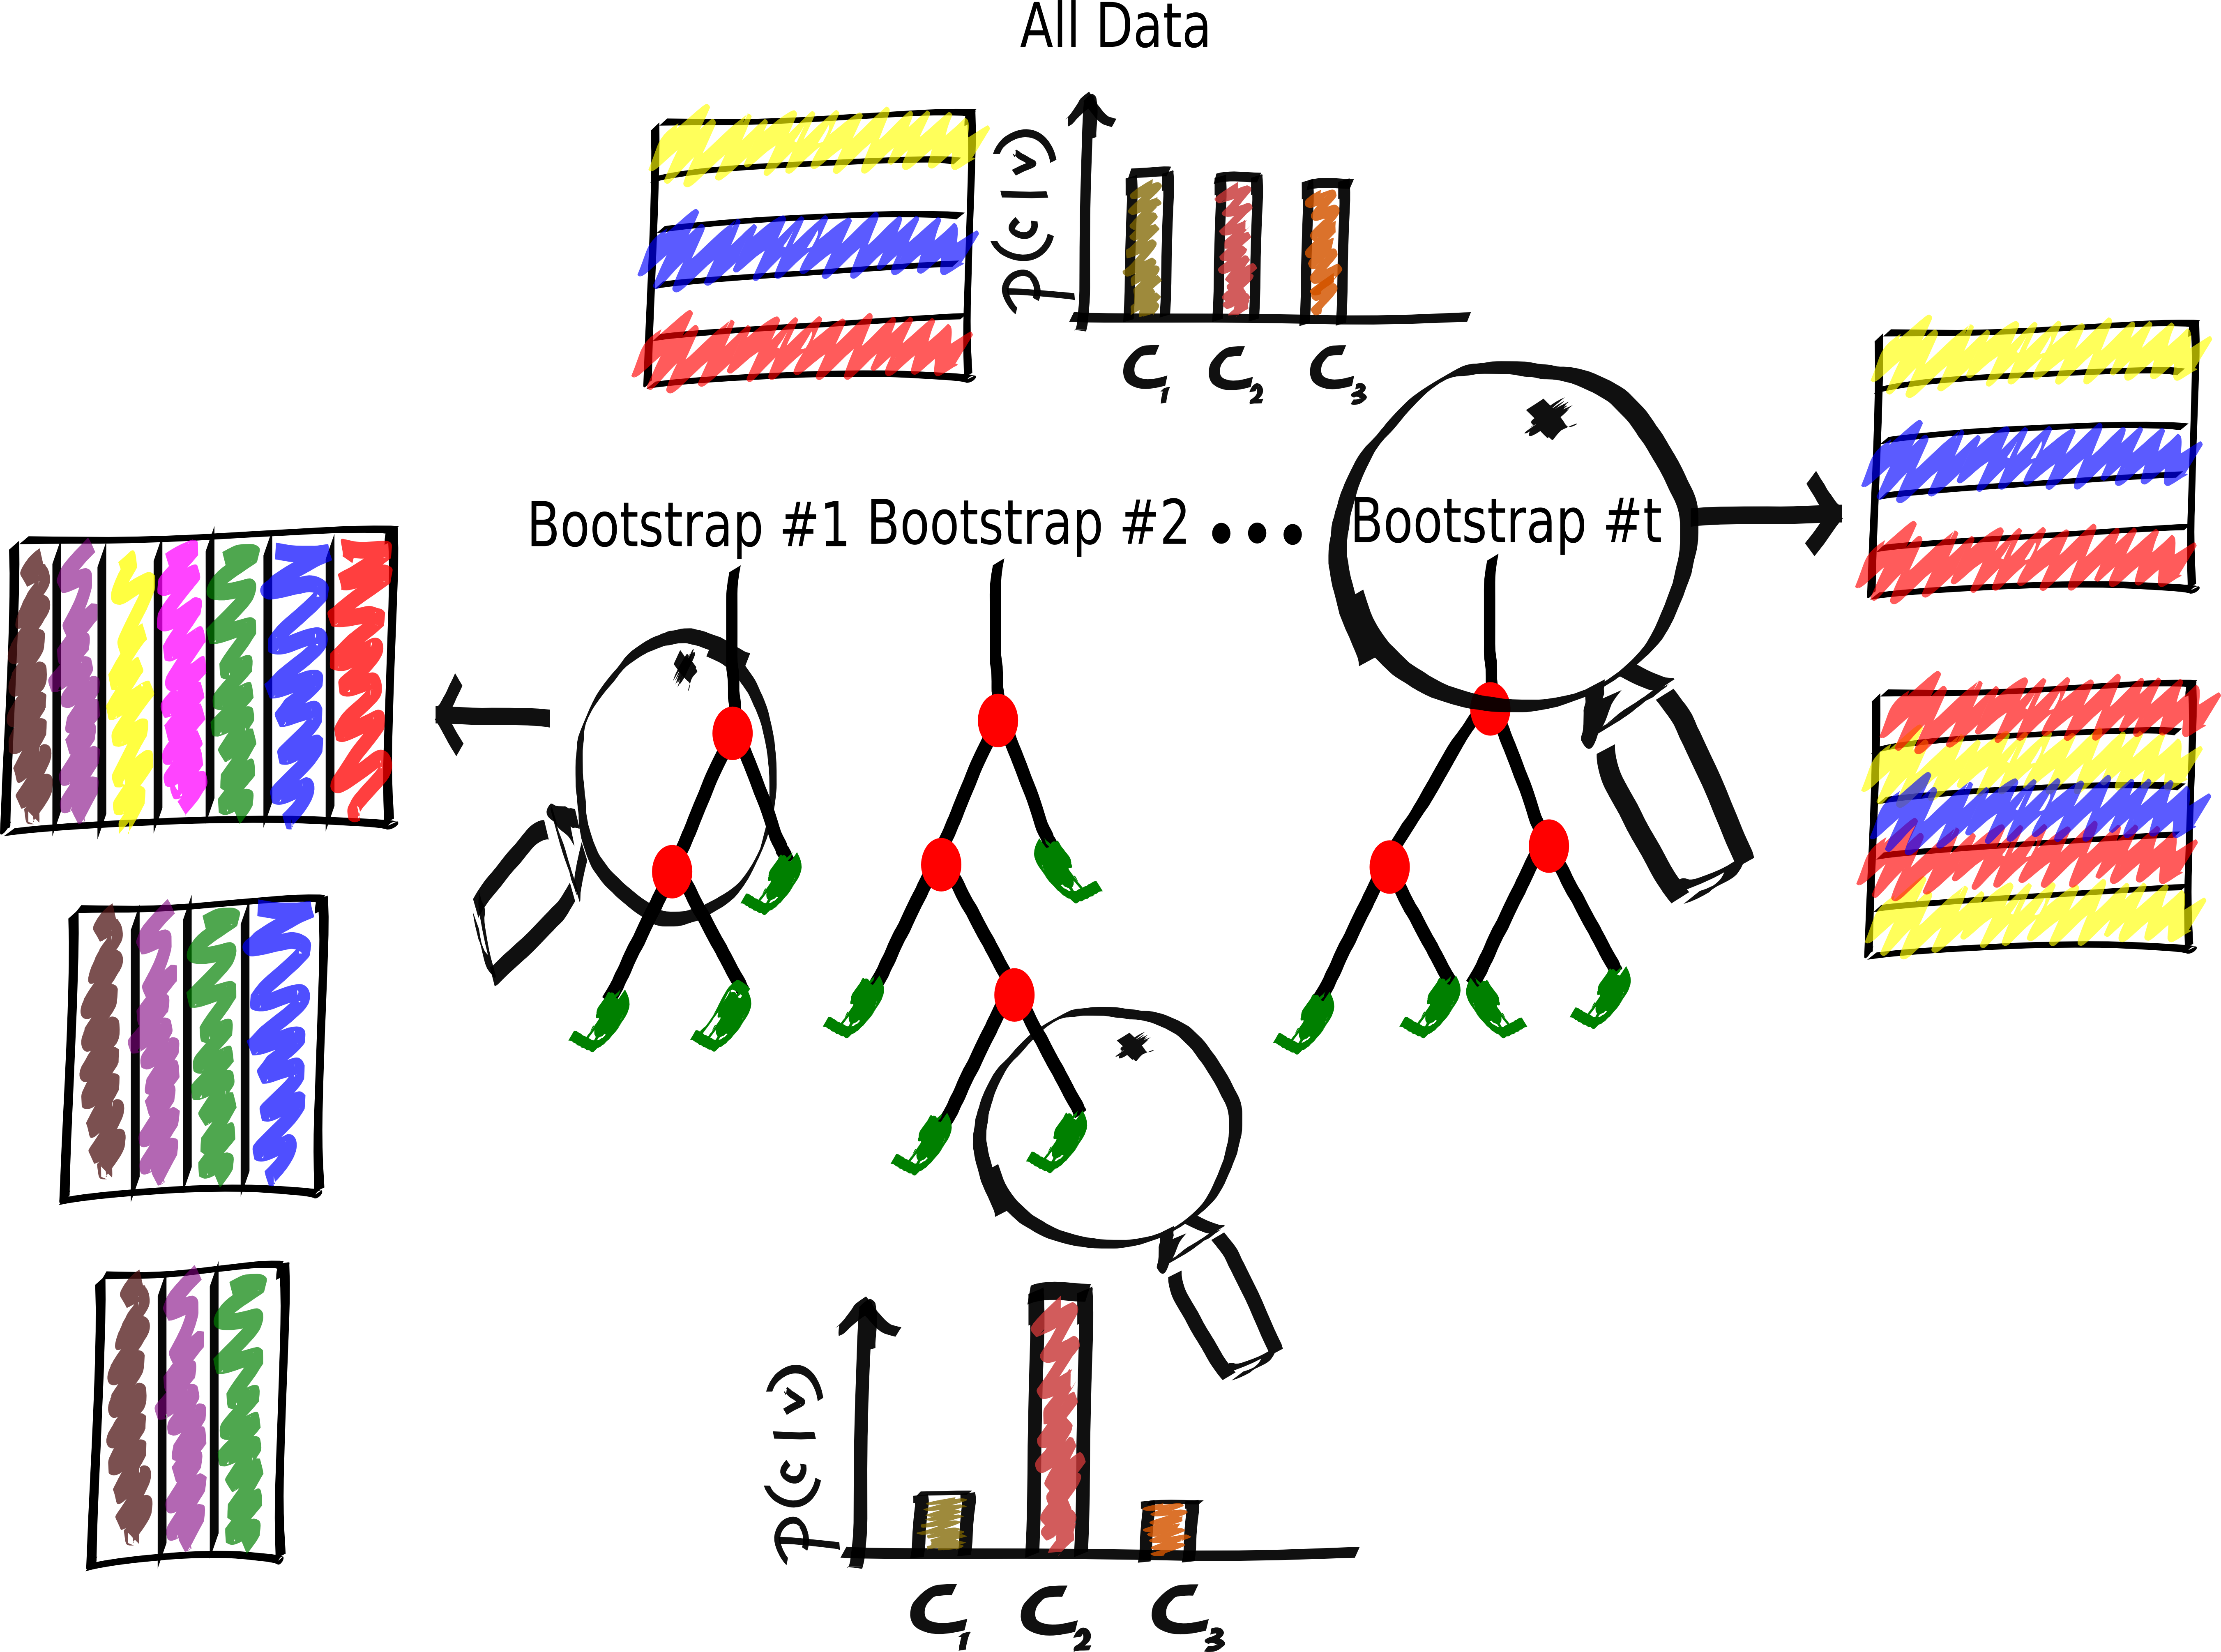
\includegraphics[width = 0.8\textwidth, height = 0.4\textheight]{Chapter2/Figures/RF_train.png}
\label{fig:rftrain}}\\
\subfloat[]{
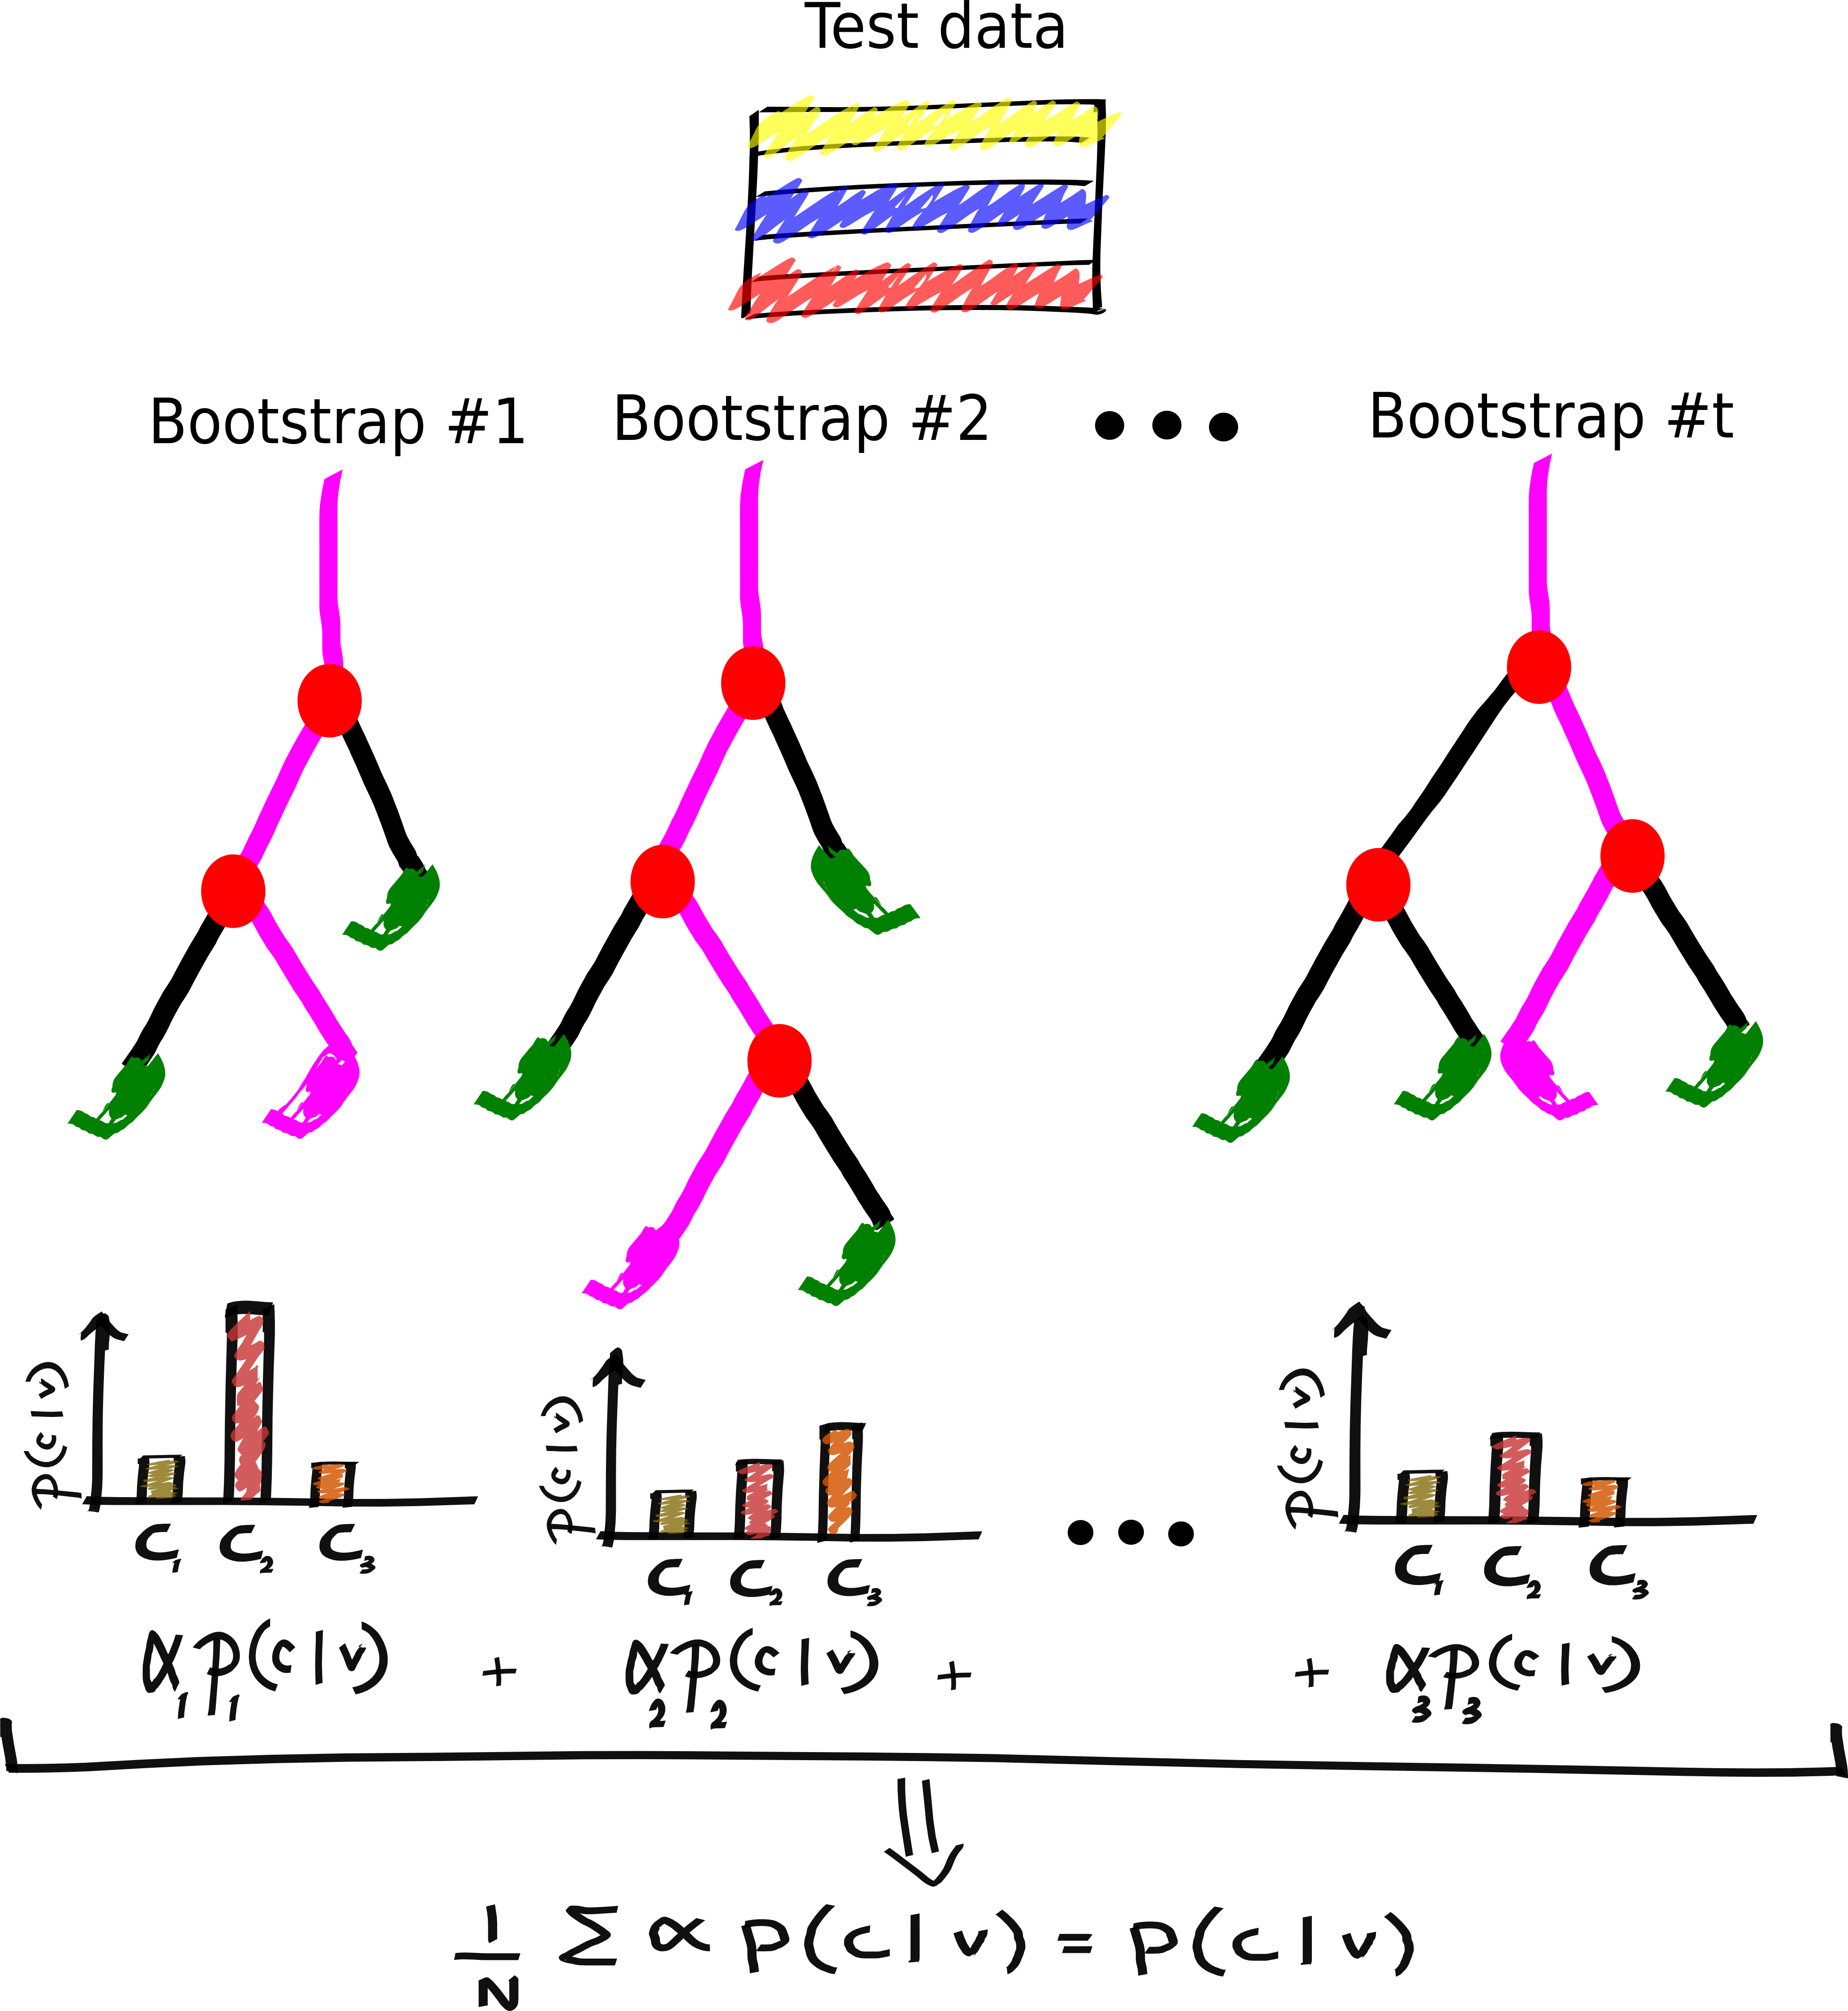
\includegraphics[width = 0.5\textwidth, height = 0.4\textheight]{Chapter2/Figures/RF_test.png}
\label{fig:rftest}}
\caption[\acl{rf} classifier]{\Ac{rf} ensemble: (a) training stage of \ac{rf} ensemble. This ensemble randomizes the training by first creating different bootstraps for training each tree in the forests. Second, at each node of the tree, it randomly considers a smaller set of feature dimensions. Each node of a tree predicts one class. (b) testing stage of \ac{rf} ensemble. A test sample is passed through all the trees and its prediction is assigned by majority voting of predicted labels of the trees.}
\label{fig:rf}
\end{figure}

 
\item[\acf{gb}] is a generalization form of \ac{adb} able to use real-value weak learners and minimize different loss functions~\cite{zheng2007general}.
\ac{gb} builds the ensemble in a greedy manner. 
It iteratively selects the best pair of real-valued weak learners and adjusts their weights so they minimize a given differentiable loss function.
\begin{subequations}
\begin{align}
\mathcal{L} & = \sum\limits_{i = 1}^{N} L(y_{i}, \varphi(x_{i})),\\
\varphi(x) & = \sum\limits_{j = 1}^{M} \alpha_{j} h_{j}(x),
\end{align}
\end{subequations}
\noindent here $h_{j}(.)$ is the weak learner and $\alpha_{j}$ is the real value weight and the aim is to minimize $\mathcal{L}$. 
A common choice for the weak learner is a decision stump or regression tree while the loss function is generally an exponential or a logarithmic loss~\cite{becker2013supervised}. 
\begin{subequations}
\begin{align}
\text{Exponential loss } \qquad L &= e^{-y_{i}\varphi(x_{i})}, \label{eq:exploss} \\ 
\text{Log loss } \qquad L &= \log(1+e^{-2y_{i}\varphi(x_{i})}).
\end{align}

\end{subequations}
This minimization can be carried out via a gradient descent or a quadratic approximation.

\item[Stacking]~\cite{wolpert1992stacked} is another way to create an ensemble from multiple base learners.
The idea is to have a meta learner which considers the predictions of the previous base learners as input for the training stage and combines them into a final decision.
Using this technique, the training data is partitioned into two sets, which we call training and validation sets. 
Each base learner is trained on the training set and its prediction on the validation set is fed to the meta learner.
Similarly, the test sample is first classified by the base learners and their prediction is passed through the meta learner in order to arrive at the final decision.
Stacking seems to avoid overfitting and improves performance when it is used with cross-validation~\cite{dvzeroski2004combining}.
This technique was used for problems such as segmentation and labeling~\cite{murphy2012machine}.
Figure~\ref{fig:stacking} shows the principal of the staking approach. 
\begin{figure}[t]
\centering
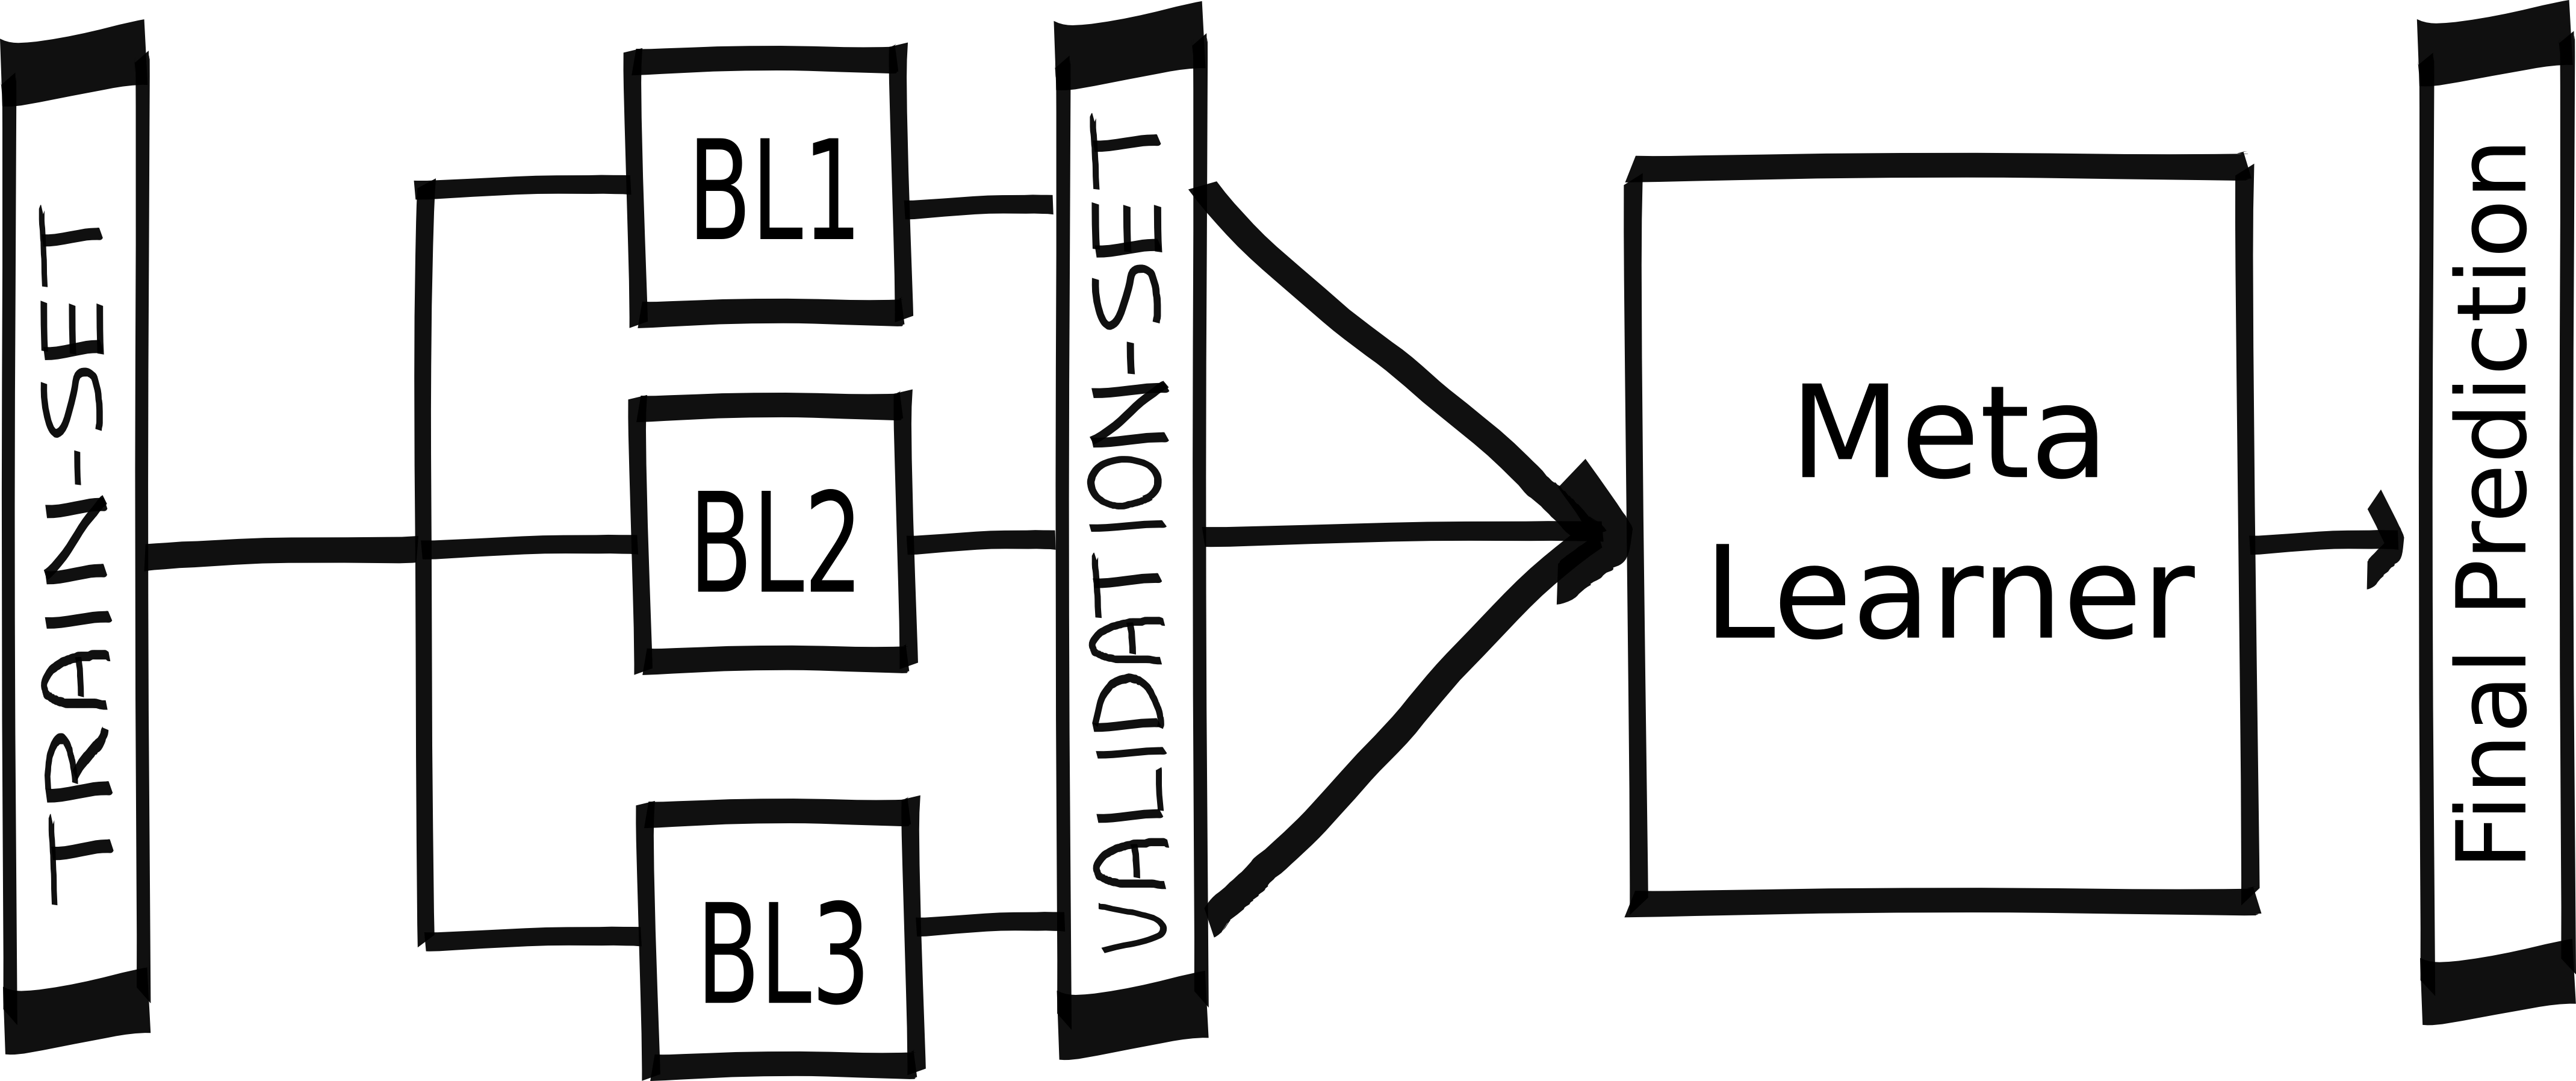
\includegraphics[width = 0.5\textwidth]{Chapter2/Figures/Stacking.png}
\caption[Stacking ensemble]{Staking ensemble approach for three base learners (BL1, BL2, and BL3). Different base learners can be combined using this method.}
\label{fig:stacking}
\end{figure}

\item[\acf{ecoc}] is an interesting way of ensemble learning, especially suitable for multiclass classification~\cite{dietterich1995solving}.
This technique allows the application of binary classifiers for multiclass classification by randomly assigning different classes to a ``super-class'' (0 or 1). 
Let us consider a 5 class classification $C \in \{A,B,D,E,F\}$, each time a set of classes is randomly assigned to one of the super-classes.
For instance, lets consider a binary classifier, where $A$ and $F$ are categorized in super-class 1 and $B$,$D$, and $E$ belong to super-class 0. 
Repeating the binary classification several times, each class will be represented by a binary code. 
This binary code states that in each binary classification, our considered class was categorized in one or the other super-class. 
Going back to our example and assuming a 5 binary classification, having a binary code $11010$ for class $F$ shows that for binary classification problems of 1,2, and 4, $F$ was assigned to super-class 1 and the rest to 0. 
Subsequently, an ensemble is created as a combination of binary classifiers.
Similarly, a test sample is classified with all the binary classifiers and receives a predicted binary code.
The predicted class is assigned based on the closest class vector to the predicted vector. 
Hamming distance is used to find a closest class vector. 
Although the classes can be assigned in a pre-designed manner to maximize their distance to each other, James~et. al~\cite{james1998error} showed that the random code works just as well as the optimal code~\cite{murphy2012machine}. 
%{\color{blue} Eventually if the created code vector is long enough, the effect of randomness is not feasible.}

\item[Weighed combination] is a very simple way of ensemble learning, and, as its name suggests, it creates a weighted combination of base learners.
Each base learner will have a strength proportional to its assigned weight.
The assigned weight can be fixed or dynamically determined.
There are different approaches to determine the base learners' weights: majority voting (plurality vote), Bayesian combination, entropy weighting and performance weighting among others~\cite{rokach2010ensemble}.
Each base learner's weight is proportional to the aforementioned measures on the validation set.
Figure~\ref{fig:LC_general} shows an ensemble based on performance weighting of three base learners (BL). 
\begin{figure}
\centering
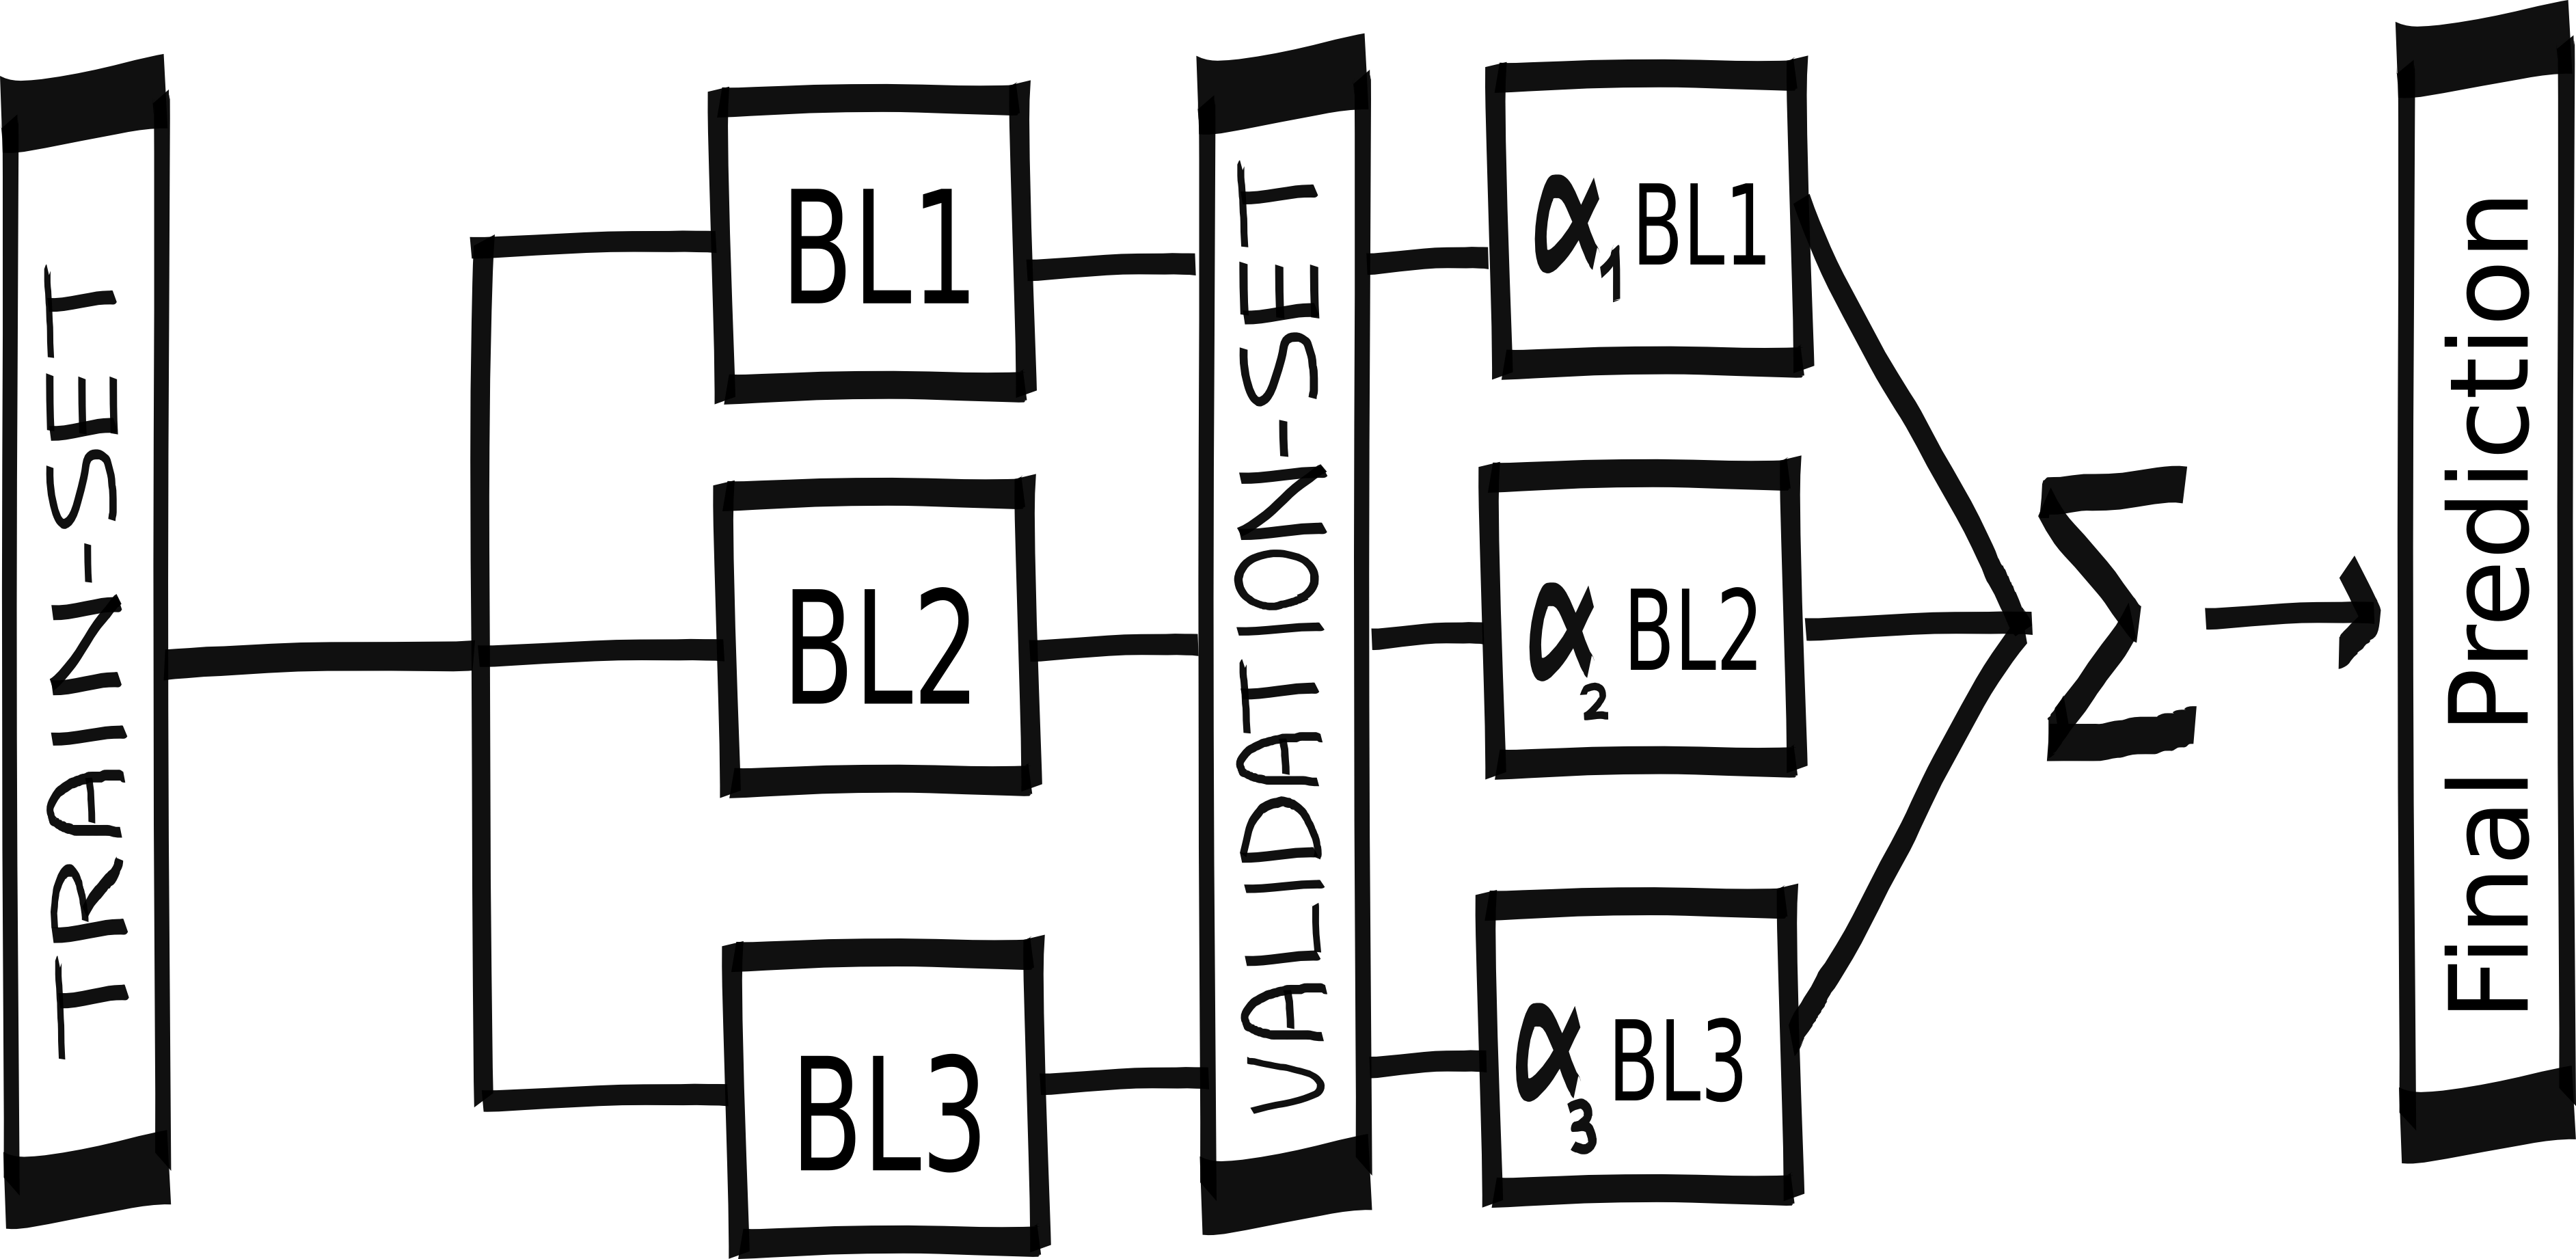
\includegraphics[width = 0.5\textwidth]{Chapter2/Figures/LC_gen.png}
\caption[Weighted Combination ensemble]{An ensemble of three base learners (BL1, BL2, and BL3, respectively) weighted by their performance on the validation.}
\label{fig:LC_general}
\end{figure} 
\end{description}



%%% Local Variables: 
%%% mode: latex
%%% TeX-master: "../thesis"
%%% End: 
